\documentclass[12pt]{article}
\usepackage{amsmath}     
\usepackage{alltt}                 
\usepackage{graphicx}
\title{Exploring the Image Processing Toolbox}
\author{
   \\Tarif Rahman
  \and
    \\Robin Jha}
\begin{document}
\maketitle
\hspace {1 cm}
\begin{abstract}
Image processing is any form of signal processing for which the input is an image, such as a photograph or video frame;
 the output of image processing may be either an image or, a set of characteristics or parameters related to the image.
 In this project we will implement different image-processing techniques in an attempt to make a tutorial which can be used 
by individuals as a tutorial.
  \end{abstract}
  \section{Introduction}
   As a part of the course requirement, COSI-177A, we were required to choose a package or library from Octave/MATLAB
that had not been covered in class. We decided to choose the MATLAB Image Processing ToolBox as we have modest familiarity with the library. Since we are not working with any specific problem we will be designing a tutorial in which we will describe the general functionalities of the toolbox as well as the undelying mathematics of these libraries.    
  \section{Functions Used}
    Image processing consists of a set of basic functions where the images has to go through a series of processes before any useful information can be extracted from it. In this section we discuss some of the features of the image processing toolbox which we used for our project.
   \subsection{Reading an Image}
     Before we do anything with the image, it needs to be read into the buffer space. To do this we execute the command below
   \[{\bf I=imread('example.tif')}\]
    \begin{figure}
    \centering
    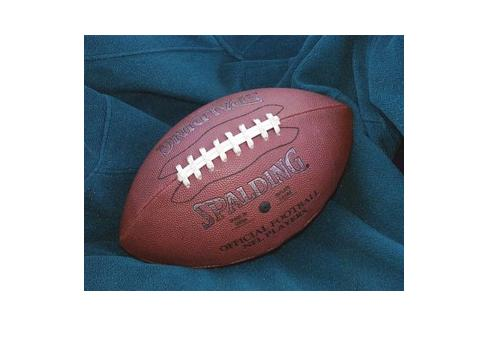
\includegraphics[scale=0.5]{football.jpg}
    \caption{The sample RGB image showing a Spalding Football}
    \end{figure}
    The imread function takes a string as input like in this example 'example.tif' is the name of the image file and it returns a matrix or a multidimensional array to the variable I. The dimensions of the array are dependent on the type of image we are dealing with. RGB images are three dimensional arrays and two dimensional arrays are usually the resultant of grayscale and black and white images. Figure 1 is a typical RGB image in which the matrix that comprises the image is three dimensional. 
   Once this command is executed, we can show the image by using imshow():
    \[ {\bf imshow(I)}\]

    \subsection{Cropping an Image}
	An image generally has many features which includes regions of interests and other regions which we might need to get rid of. Imcrop in matlab is an interactive image cropping tool which lets you do that. 
   \[{\bf I2 = imcrop('example.tif')}\]
    \clearpage
    \begin{figure}
       \centering
      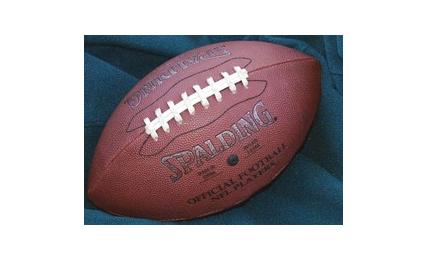
\includegraphics[scale=0.5]{footballcrop.jpg}
      \caption{Image after cropping Figure 1}
      \end{figure}
    The command above displays the image 'example.tif' in a figure window and creates a cropping tool associated with that image. Example.tif can be a grayscale image, a truecolor image, or a logical array. The cropped image returned, I2, is of the same type as example.tif.

   \subsection{Histogram Equalization}
    Histogram Equalization is used to adjust the histogram of the image. As a result of this operation areas of local lower contrast gains a higher contrast. To extract useful information using this method, the intensities of the different channels are distributed evenly throughout on the histogram \cite{Mathworks3}.However, the limitation of this method is that is can decrease the intensity of the actual signal while increasing the background noise. The syntax in matlab is as follows
 \[ {\bf I = imread('example.tif');}\]
  \[{\bf J = histeq(I);}\]
       \clearpage
       \begin{figure}
       \centering
      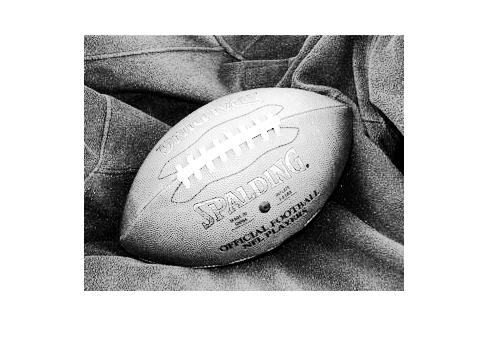
\includegraphics[scale=0.5]{footballhisteq.jpg}
      \caption{Image after applying histogram equalization on Figure 1}
      \end{figure}

   \subsection{RGB To Grayscale}
   Color images are often a result of a combination of several color channels. For example, RGB images are composed of three independent channels for red,blue and green which form the primary color components. These colors in the image can be converted to a grayscale image by calculating the effective luminance of the color values \cite{Mathworks2}. A shade of gray matching this brightness is then created by retaining the luminance and eliminating the hue and saturation information.
  \[{\bf I2 = rgb2gray('example.tif')}\]
  
   \clearpage
   \begin{figure}
   \centering
   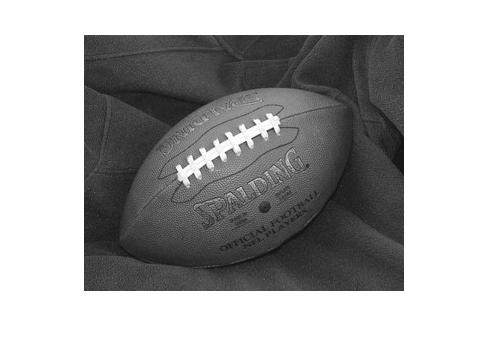
\includegraphics[scale=0.5]{footballgray.jpg}
   \caption{The sample grayscale image of Figure 1}
   \end{figure}
   
    \begin{verbatim}
	t=imread('football.jpg');
	dims=size(t);
	y=[];
	for j=1:dims(1)
      for k=1:dims(2)
            y(j,k,1)=0.299*t(j,k,1) + 0.587*t(j,k,2) + 0.114*t(j,k,3);
            y(j,k,2)=0.299*t(j,k,1) + 0.587*t(j,k,2) + 0.114*t(j,k,3);
            y(j,k,3)=0.299*t(j,k,1) + 0.587*t(j,k,2) + 0.114*t(j,k,3);
          end
    	end
	imshow(y)
	}
	\end{verbatim}
    
   \subsection{Noise Reduction Using Median Filter for GrayScale Images}
   Images usually comes with a certain amount of noise in them. Noise in this case means unwanted data which has no meaning. To rectify this problem and extract useful information it is often desirable to perform some kind of noise reduction for which there are various techniques in Matlab.The one we used is called median filtering.Noise reduction is a common procedure to improve the results of later processing to follow, such as edge detection, on an image. Median filtering is very widely used in image processing because it tends to remove the noise while preserving the edges.
    
      \[{\bf I2 = medfilt2('example.tif')}\]
      \begin{figure}
       \centering
      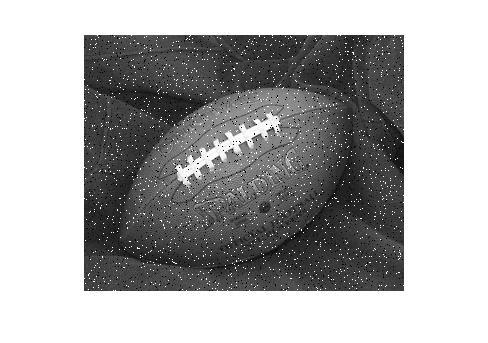
\includegraphics[scale=0.5]{impure.jpg}
      \caption{Image with salt and pepper noise}
      \end{figure}
       \clearpage
       \begin{figure}
       \centering
      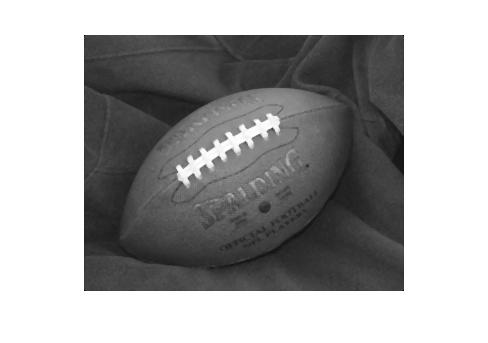
\includegraphics[scale=0.5]{footballmedfil.jpg}
      \caption{Image after applying median filter on Figure 5}
      \end{figure}
       
\subsection{Edge Detection for Feature Extraction}
    Edge detection is a complex task and becomes more difficult when the intensity difference between neighbouring pixels is small.The concept of edge detection is used in context of feature extraction where the main aim is to identify the points undergoing sharp transform in image brightness. The main idea behind it is to capture the important details that might not be evident from the original image. The result of applying an edge detector to an image may lead to a set of connected curves which outlines the boundaries of objects and discontinuities in the surface orientation. In our case we used the Canny method. 
\begin{quote}
The Canny method finds edges by looking for local maxima of the gradient of example.tiff. The gradient is calculated using the derivative of a Gaussian filter. The method uses two thresholds, to detect strong and weak edges, and includes the weak edges in the output only if they are connected to strong edges. This method is therefore less likely than the others to be fooled by noise, and more likely to detect true weak edges \cite{Mathworks}.
\end{quote}
\[{\bf BW = edge(example.tif,'canny')}\]
      \clearpage
      \begin{figure}
       \centering
      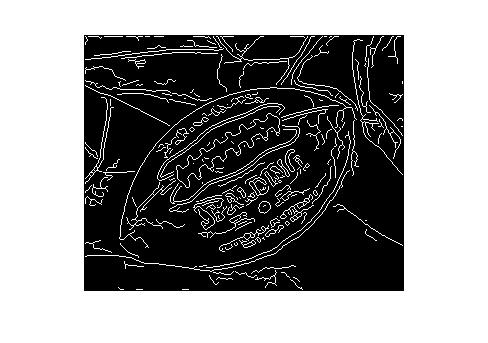
\includegraphics[scale=0.5]{footballcanny.jpg}
      \caption{Image after applying canny method on BW copy of Figure 1}
      \end{figure}
     
The edge function takes a grayscale or a binary image example.tif as its input, and returns a binary image BW of the same size as example.tif, with 1's where the function finds edges in example.tif and 0's in the rest of the places.

An edge in an image can point in any direction.As a result of this Canny uses four different filters to detect the vertical, horizontal and the diagonal edges in the image. The edge detection operators like Sobel, Roberts, etc return a value for the first derivative in the horizontal direction \[G_x\] and the vertical direction \[G_y\] From this the edge gradient and direction can be determined by the formula below:
\[G=\sqrt{G^2_x+G^2_y}\]
\[\theta=\arctan(G_y/G_x)\]
In the next step the edge direction angle is rounded off to one of the four angles in the four different directions with an angle measure at 0, 45, 90 and 135 \cite{Mathworks4}.

Once the directional angles are determined non-maximum suppression is performed to trace the edge in the edge direction. In this process the pixel values which is not an edge is set to 0 thus giving a thin line in the output image \cite{Mathworks4}.

Finally, in the last step a threshold value is used to eliminate the edge pixels from others. Any pixel in the image that has a value greater than the threshold is presumed to be an edge pixel, and is marked as such immediately while ignoring the rest \cite{Mathworks4}.

\section{Matlab Code}
\begin{verbatim}
image=imread('football.jpg'); % reading an image
subplot(2,4,1)
imshow(image) % showing the image
image_gray=rgb2gray(image);   % converting the image to a gray scale image
distorted_image=imnoise(image_gray,'salt & pepper'); % adding noise to the gray scale image
restored_image=medfilt2(distorted_image); % filtering the distorted image
subplot(2,4,2), imshow(image_gray) % showing the gray scale image
subplot(2,4,3), imshow(distorted_image) % showing the distorted image
subplot(2,4,4), imshow(restored_image) % showing the restored image
image_hist=histeq(image_gray); % showing the result of histogram equalization
subplot(2,4,5),imshow(image_gray)% showing the gray scale image
subplot(2,4,6),imshow(image_hist) % showing the histogram equalized image
image_edge=edge(image_gray,'canny');
subplot(2,4,7),imshow(image_gray) % showing the gray scale image
subplot(2,4,8),imshow(image_edge)% showing the gray scale image with edges detected
\end{verbatim}

\begin{thebibliography}{9}

\bibitem{Mathworks} ,
\emph{MathWorks - MATLAB and Simulink for Technical Computing},
Find Edges in Grayscale Image - MATLAB,
Mathworks- Web. 18 Apr. 2011.

\bibitem{Mathworks2} ,
\emph{MathWorks - MATLAB and Simulink for Technical Computing},
Convert RGB Image or Colormap to Grayscale - MATLAB,
Mathworks- Web. 18 Apr. 2011.

\bibitem{Mathworks3} ,
\emph{MathWorks - MATLAB and Simulink for Technical Computing},
Enhance Contrast Using Histogram Equalization - MATLAB,
Mathworks- Web. 18 Apr. 2011.

\bibitem{Mathworks4} ,
\emph{Green, Bill. "Canny Edge Detection Tutorial."},
 Personal Websites - Office of Information Resources and Technology. Web. 03 May 2011,
\begin{verbatim}
http://www.pages.drexel.edu/~weg22/can_tut.html 
\end{verbatim} 
\end{thebibliography}

\end{document}
